\documentclass[12pt,titlepage]{report}

\usepackage{float}
\usepackage[T1]{fontenc}
\usepackage[utf8]{inputenc}
\usepackage[french]{babel} 
\usepackage{amsmath}
\usepackage{amssymb}
\usepackage[top=1.5cm, bottom=1.5cm, left=1.5cm, right=1.5cm]{geometry}
\usepackage{graphicx}
\usepackage{float}
\usepackage{multicol}
\usepackage{lipsum}
\usepackage{ragged2e}
\usepackage{hyperref}
\usepackage{enumitem}
\usepackage{eurosym}
\usepackage{indentfirst}
\usepackage{minted}
\usepackage{titlesec}
\usepackage{pifont}
\usepackage{url}
\usepackage{epsf}
\graphicspath{ {images/} }

\begin{document}

\begin{titlepage}
\newcommand{\HRule}{\rule{\linewidth}{0.5mm}}
\center
\includegraphics[scale=0.4]{ul_logo.jpeg} \\[0.6cm]
\includegraphics[scale=1.2]{telecom_nancy.png} \\[0.2cm]
\HRule
{ \huge \bfseries PPII - Projet Pluridisciplinaire d'Informatique Intégrative 2 \\
        \Large Plus petit parcours voiture électrique\\[0.15cm] }
\HRule \\[1cm]
{\LARGE \textbf{Responsables du module :}}
\vskip 0.1cm
{\Large 
Oliver FESTOR \\ 
} 


\vspace{1cm}
{\LARGE \textbf{Équipe projet}} \\ 
\vspace{0.1cm}
\Large Lucas ARIES \\
Paul DEVEAUX, \\ 
Théo HORNBERGER \\
Terry TEMPESTINI\\
\vspace{3cm}
    
2022/2023 \\ [1cm]
\end{titlepage}

\tableofcontents
% ---------------------------------- TABLE DES MATIERES -------------------------
\clearpage
% ---------------------------------- Début document ----------------------------------
\chapter{Gestion de projet}

\section{Réunion et Planification}
\textbf{Les comptes rendus de réunion sont disponibles dans la partie annexe.} \\ \\ 

La planification du projet a été réalisée à l'aide d'un diagramme de Gantt, dont le rôle principal était de s'assurer que nous ne prenions pas trop de retard. \\
Mais aussi à l'aide des différentes réunions qui ont rythmé ce projet. Les réunions avaient pour objectif de parvenir à un accord sur la compréhension du problème et de la solution nécessaire, de mener ensemble des séances de brainstorming pour trouver la réponse la plus cohérente et efficace possible, ainsi que de s'assurer que chaque membre du groupe atteigne ses objectifs et progresse dans la bonne direction.

\section{Répartition et rythme de travail}

Le travail a été réparti en objectifs classés selon leur importance et leur urgence afin de déterminer l'organisation du travail. \\

\begin{center}
\includegraphics[scale=0.35]{taches.png} \\    
\end{center}

Le travail de développement a été réparti en 4 grands axes majeurs : la récupération des données, la recherche de chemin, l'interface graphique et la simulation. La dernière partie du projet, le mode simulation, a été mis en suspens dès le début afin de permettre à la première partie de fonctionner correctement. L'objectif était d'avoir un programme fonctionnel, sans aucun bug, performant et utilisable en conditions réelles.  \\
Une fois l'application de base fonctionnelle, nous avons commencer à travailler sur la partie simulation.\\

La récupération des données étant la tâche la plus urgente pour pouvoir bien avancer dans les autres, celle-ci devrait être réalisée en première  \\
Le développement de l'algorithme étant la tâche la plus importante il y a eu  2 personnes y étant assignée contrairement aux autres tâches. Il y a également eu plus de recherche sur celle-ci pour trouver la solution idéale. \\
L'interface graphique étant une part de travail conséquente mais ni urgente ni importante, a été réalisée durant toute la durée du projet. \\

\section{Analyse Post-Mortem}

Nous avons rencontré plusieurs difficultés lors de notre travail, notamment lors de la récupération des stations au format CSV. Au départ, nous avions un fichier contenant plus de 50 000 lignes, mais nous avons constaté la présence d'un grand nombre de doublons. Nous avons donc créé un programme Python afin de les supprimer, ce qui nous a laissé avec environ 17 000 lignes. De plus, nous avons également rencontré des problèmes avec le format des données, notamment la présence de caractères spéciaux qui ont provoqué des plantages de l'interface graphique. Nous avons dû résoudre ce problème.
\\ \\
Concernant l'algorithme de recherche de chemin, nous somme rapidement arrivé à un résultat mais il pouvait être très lent sur certains itinéraires, et il y avait de nombreuses fuites mémoires.
L'implémentation de la file de priorité a été réécrite plusieurs fois : C'était tout d'abord un simple arbre binaire non équilibré. L'algorithme mettait trop de temps lorsque le chemin était long, donc une implémentation d'un arbre binaire équilibré a été choisi. Pour cela, nous avons d'abord décidé de faire un arbre bicolore. L'algorithme marchait mais il y avait de nombreuses fuites mémoires qui étaient très compliqué à résoudre à cause de la taille des fonctions d'insertion et de suppression (trouver d'où venaient les fuites était trop laborieux). Nous avons donc décidé de choisir une implémentation plus simple, et qui a été vu en cours : l'arbre avl.
\\ \\
Parlons maintenant de l'interface graphique, qui a été l'une de nos principales difficultés. Sa réalisation a été complexe et chronophage. En effet, l'implémentation des différentes méthodes et signaux ont du être changé et adapté plusieurs fois afin de correspondre à la vision que nous en avions au préalable. Heureusement, nous avions anticipé cela en confiant à Théo la tâche de s'en occuper dès le début du projet, ce qui nous a permis d'obtenir un résultat satisfaisant dans les délais.
\\ \\
Nous sommes également satisfaits d'avoir effectué une recherche approfondie sur les algorithmes et les structures de données, car nous avons obtenu des temps de calcul très raisonnables, d'environ 0.3 seconde. Cela confirme que nos choix de résolution du problème étaient judicieux, d'autant plus que notre réalisation très basique de l'algorithme de Dijkstra prenait environ 40 secondes (possible de l'améliorer, mais pas nécessaire car servait juste de test).
\\ \\
Cependant, nous avons rencontré quelques difficultés tout au long du projet, notamment des problèmes de communication. De plus, le calcul de la distance entre deux stations renvoyait un entier alors qu'un nombre décimal était nécessaire. Finalement, le plus gros problème a été la période des examens qui est tombée vers la fin du projet, ce qui nous a contraints à réaliser la majeure partie du travail dès le départ. Cela a ralenti la résolution des différents problèmes, des bugs et la rédaction du rapport sur la fin.


\newpage
\chapter{Rapport}

\section{Dataset}
Les données ont été récupérées au format CSV pour plusieurs raisons :
\begin{enumerate}
    \item La performance : La récupération d'informations à partir d'un fichier CSV est très rapide, contrairement par exemple au format JSON, avec environ 17 000 lignes traitées en 0,025 secondes.
    \item Le stockage : Le format CSV permet facilement de retirer les données non pertinentes, ce qui a permis de réduire la taille du fichier contenant toutes les stations de 45 Mo à 2,8 Mo.
    \item La facilité de traitement dans un programme en langage C : Il est simple de lire un fichier CSV et de remplir les structures de données souhaitées dans un programme en langage C. \\
    La seule difficulté rencontrée a été la présence du caractère délimiteur ';' dans le nom de certaines stations. Il a donc fallu détecter si c'était le cas, en prenant en compte que les noms contenant ce caractère étaient encadrés par des guillemets (" ").
\end{enumerate}

Nous avons veillé à ne lire le fichier qu'une seule fois et à générer une liste remplie de la structure correspondant à une station ou une voiture en langage C. Cela permet d'accéder rapidement à une station pendant l'exécution de l'algorithme. Nous avons choisi une liste car elle est rapide en lecture mais lente en modification. Cependant, nous n'allons jamais modifier la liste et nous allons souvent y accéder. Par conséquent, ce choix est pertinent pour optimiser notre algorithme.

\section{Position géographique de la station}

Une des difficultés rencontrées fut la présence de deux formats de données représentant la position géographique de la station : les coordonnées x, y et la latitude, longitude. Nous avons opté pour la deuxième méthode, car elle est plus largement utilisée et nous n'avions pas d'information sur le référentiel utilisé dans la première méthode. Cependant, cela signifiait que nous devions désormais convertir les deux types de coordonnées en distances pour les comparer. \\ \\ 

Pour ce faire plusieurs méthodes était disponible a nous toujours en prenant en compte le soucis de performance \\ 
source: \href{http://villemin.gerard.free.fr/aGeograp/Distance.htm}{Villemin gerard - calcul de distance} \\
Deux méthode nous sont donc parvenu comment étant intéressantes : \\
\begin{enumerate}
    \item La première méthode utilisait le théorème de Pythagore, ce qui offrait l'avantage d'une performance accrue avec peu d'opérations complexes et donc un temps d'exécution rapide. Cependant, l'inconvénient était la perte de précision sur les distances pour de longs trajets, pouvant varier de quelques kilomètres.
    \item La seconde méthode s'appelle la formule de Haversine. Son avantage réside dans sa précision, qui est bien supérieure à celle de l'autre solution. Cependant, son inconvénient est qu'elle nécessite plus d'opérations et donc entraîne un temps d'exécution plus long.
\end{enumerate}
Le choix de la solution a donc été basé sur la durée d'exécution de la formule de Haversine. Nous avons réalisé des tests et obtenu comme résultat : pour 1 000 000 calculs = 0,139 secondes. Nous avons donc jugé cela suffisamment rapide et avons choisi cette solution.



\section{Etat de l'art}
Nous allons dans un premier temps analyser les différentes applications qui mettent en œuvre des solutions à notre problème, puis dans un second temps nous verrons les solutions envisageables avec les avantages et inconvénients de chaque algorithme.

\subsection{Applications étudiées}
Les principales applications qui font face à ce problème sont les systèmes de navigation. En effet, il peut être important pour ces applications de trouver en un temps raisonnable le plus court chemin entre 2 points en passant par un certain nombre de stations.\\
\\
Ce problème se pose également dans d’autres circonstances, par exemple dans les réseaux de télécommunications (pour transmettre des données), dans la conception de circuits électroniques (optimisation des routes et des connexions entre les composants électroniques) ou encore dans les robots (robots autonomes, de nettoyages).\\
\\
Nous allons étudier à travers un tableau les différentes solutions mises en place pour faire face à ce problème :

\begin{center}
\begin{tabular}{|p{4cm}|p{8cm}|p{3cm}|}
\hline
\textbf{Domaine} & \textbf{Problème} & \textbf{Solution} \\ \hline
Systèmes de navigation & Trouver le plus court chemin entre deux points & Dijkstra et A* \\ \hline
Réseaux de télécommunications & Chemin le plus court en passant par des points & Algorithme de Johnson, saut de point \\ \hline
Circuits électroniques & Optimiser les routes et les connexions entres les composants & Algorithme de RRT, Probabilistic Roadmap \\ \hline
Robots & Planifier les mouvements de robots autonomes & Dijkstra \\ \hline
Planification de la production & Planifier les mouvements de matières premières, produits finis & Algorithme de Bellman-Ford, A* \\ \hline
Jeux vidéos & Jeux de stratégie, itinéraires & Algorithme de Lee-Moore, A* \\ \hline
\end{tabular}
\end{center}

Nous avons pu voir les différentes solutions mises en place pour faire face à des problèmes similaires. Le choix de l’algorithme dépend du contexte et des contraintes du problème à traiter ainsi que des performances requises. La précision des résultats donnés entre également en jeu pour choisir celui qui convient le mieux.

\subsection{Algorithmes utilisés}
Parmi ces solutions, A* et Dijkstra apparaissent comme les algorithmes les plus adaptés. En effet, dans notre cas, il s’agit d’un graphe complet non orienté, c’est pourquoi les méthodes itératives utilisées par A* et Dijkstra permettent de parcourir efficacement et dans un temps raisonnable tous les nœuds du graphe. Ils permettent aussi de prendre en compte les poids des arêtes.\\
\\
Critères utilisés pour choisir les algorithmes :
\begin{itemize}
\item Complexité algorithmique (besoin de rapidité)
\item Complexité mémoire (ne doit pas nécessiter un espace mémoire trop grand)
\item Précision requise (approche de la solution optimale)
\item Contraintes d’autonomie de la voiture
\item Structure du graphe (graphe pondéré complet non-orienté)
\end{itemize}

\subsubsection{Algorithme de Dijkstra :}

Pour implémenter Dijkstra, nous avons transformé le graphe complet en un graphe sur lequel chaque point est relié uniquement aux autres points atteignables par l’autonomie de la voiture. Afin de ne pas avoir à stocker la matrice des distances, qui est une matrice carrée (ici d’ordre 17 000) nous avons décidé de calculer les sommets adjacents à chaque itération. Ce choix affecte les performances en augmentant le temps de calcul pour un trajet mais est plus efficace que de calculer et stocker la matrice des distances.\\
\\
Avantages de Dijkstra :
\begin{itemize}
\item Garanti de trouver le chemin le plus court dans un graphe pondéré.
\item Ne nécessite pas de fonction heuristiques pour fonctionner.\\
\end{itemize}

En ce qui concerne la complexité de Dijkstra, dans notre cas (graphe complet), est en O(n²) avec n le nombre de nœuds du graphe. La complexité est relativement élevée ce qui rend le temps de calcul assez long.

\subsubsection{Algorithme A* :}

L’algorithme A* est adapté à notre problème car il permet de donner un résultat exact avec des performances bien meilleures que Dijkstra. Dans notre cas, nous avons utilisé l’arbre pondéré comme structure de données permettant d’établir facilement la liste des priorités.\\
\\
Avantages de A* :
\begin{itemize}
\item Plus rapide que Dijkstra dans des graphes de grande taille car utilise des heuristiques pour guider la recherche.
\item Plus flexible que Dijkstra, il permet de spécifier la fonction heuristique pour tenir compte de la distance restante jusqu’à la fin.\\
\end{itemize}

Pour ce qui est de la complexité de A*, celle-ci est moins élevée que Dijkstra, avec dans le pire des cas O(n) avec n le nombre de nœuds. Cette complexité est plus adaptée pour garantir un temps de calcul rapide.


\section{Implémentation}

Nous avons décidé d’implémenter ces deux algorithmes et de comparer leur efficacité sur des données réelles. L’algorithme le plus efficace sera utilisé et optimisé pour permettre d’éviter les files dans les stations. La simulation sera également faite sur cet algorithme.


\subsection{Simplification du graphe}

Comme expliqué dans l’énoncé, toutes les stations sont reliées entre elles. 
Ainsi, le graphe obtenu est un graphe complet. Ce fait pose deux problèmes :
Tout d’abord, le chemin le plus court est d’aller directement d’un point A à un point B puisqu’ils sont forcément reliés. Ce trajet direct n’est pas possible pour une voiture électrique lorsque la distance est trop grande, donc inutile.
Le stockage des distances se feraient dans une matrice de de dimension n*n, avec n le nombre de stations. Si l’on utilise des entiers afin de représenter les distances, qui ont chacun une taille de 4 octets, la taille de la matrice sera de n²*4 octets. Sachant que l’on possède un dataset comportant 17000 stations, cela nous fera une matrice comportant $2,89*.10^8$  entiers, soit 1,56 Giga-octets.

\includegraphics{images/schemas/calcul_distance_time.png}\\

Sachant que notre dataset possède à peu près 17000 stations, cela prendrait 49 secondes à calculer les distances entre chaque station. 
Il n'est donc pas possible de précalculer les distances entre chaque stations et de les stocker. Nous avons donc décidé de calculer la distance à chaque fois que nous en avons besoin.
\\

Les stations qui peuvent être atteintes à partir d'une certaine station sont calculées grâce aux paramètres du véhicule : Sa batterie et sa consommation. Ainsi, la distance maximale que le véhicule pourra parcourir en une seule fois est :
\[dmax = \frac{batterie}{consommation}\]

Afin d'offrir plus de choix à l'utilisateur, il peut choisir un seuil minimal pour laquelle la batterie ne devra pas dépasser. Ainsi le calcul change légèrement :
\[dmax = \frac{batterie}{consommation} - \frac{batterieMin}{consommation}\]

Nous avons calculé la distance maximum qu'une voiture peut effectuer en un seul trajet, mais il faut aussi préciser une distance minimum, ou le trajet calculé passera par un grand nombre de bornes qui sont à de très petites distances l'une de l'autre.\\\\

\includegraphics[scale=0.9]{images/schemas/schema_distance_petite.png}\\
Dans ce trajet, l'utilisateur part de A et veut aller à Z. Il n'est pas utile de s'arrêter sur B et C.

L'utilisateur pourra donc choisir à partir de quelle batterie il veut s'arrêter sur une borne, appelé batterieMax.
\[dmin = \frac{batterie}{consommation} - \frac{batterieMax}{consommation}\]
\\
L'utilisateur doit aussi pouvoir choisir combien de temps au maximum (tmax) il souhaite attendre sur une borne. Sa batterie ne sera donc peut-être pas rechargée à 100\% à chaque fois. Ainsi, il faut calculer à chaque station la batterie de la voiture avant la recharge et après la recharge.
\\
\[batterie Avant Charge = batterie Avant Trajet - distance Trajet * consommation\]
\[batterie Apres Charge = min(tmax/60 * puissance Station + Batterie Avant Charge, batterieMax)\]
\\
Les distances dmin et dmax sont donc calculées à partir de la batterie après charge :
\[dmax = \frac{batterieApresCharge}{consommation} - \frac{batterieMin}{consommation}\]
\[dmin = \frac{batterieApresCharge}{consommation} - \frac{batterieMax}{consommation}\]
\\
L'utilisateur peut également choisir de ne s'arrêter que sur des stations qui sont gratuites.
\\\\

\subsection{Algorithme A*}

L'algorithme A* utilise différentes structures de données afin de fonctionner, notamment une liste avec priorité, que l'on appelle l'open list, afin de gérer quelles noeuds doivent être traités avant les autres (calculées grâce à une heuristique).

La file de priorité étant une structure de données abstraite, elle peut être implémentée par plusieurs autres structures. Les plus courantes sont : Les arbres binaires, la liste chaînée triée, le tas de fibonacci et les tas binomiaux.
\\
\begin{center}
\begin{tabular}{|p{4cm}|p{6cm}|p{6cm}|}
\hline
\textbf{Structure} & \textbf{Avantages} & \textbf{Inconvénients} \\ 
    \hline 
        Liste chaînée triée & 
        \begin{itemize}[leftmargin=*]
            \item Trouver le minimum en O(1)
            \item Facilité d'implémentation
        \end{itemize} & 
        \begin{itemize}[leftmargin=*]
            \item Suppression du minimum en O(n)
            \item Insertion en O(n)
        \end{itemize}\\ 
    \hline
        Arbre binaire & 
        \begin{itemize}[leftmargin=*]
            \item Insertion et suppression en O(log n)
            \item Trouver le minimum en O(h)
            \item Facilité d'implémentation
        \end{itemize} &
        \begin{itemize}[leftmargin=*]
            \item L'équilibrage de l'arbre peut être complexe et ralentir l'insertion et la suppression
        \end{itemize}\\ 
    \hline
        Tas de Fibonnacci & 
        \begin{itemize}[leftmargin=*]
            \item Insertion et suppression en O(log n)
            \item Utilise moins d'espace qu'un arbre binaire
            \item Trouver le minimum en O(1)
        \end{itemize} &
        \begin{itemize}[leftmargin=*]
            \item Implémentation complexe
            \item Recherche du minimum en O(n) dans le pire cas
        \end{itemize}\\ 
    \hline
        Tas binomial &
        \begin{itemize}[leftmargin=*]
            \item Insertion et suppression en O(log n)
            \item Trouver le minimum en O(log n) dans le pire cas
            \item Equilibrage garanti
            \item Utilise moins d'espace qu'un arbre binaire
        \end{itemize} &
        \begin{itemize}[leftmargin=*]
            \item Implémentation complexe
        \end{itemize}\\ 
    \hline
\end{tabular}
\end{center}

En raison de sa simplicité d'implémentation et de sa performance la solution de l'arbre binaire a été choisi.\\
Afin de garantir l'équilibre de l'arbre, nous avons envisagé d'implémenter un arbre AVL ou un arbre bicolore. Le choix de l'arbre bicolore a d'abord été choisi, mais a ensuite été abandonné à cause de trop nombreuses fuites mémoires dans les fonctions d'insertion et de suppression. Il était trop compliqué de résoudre ces problèmes dû à la complexité et la taille de ces fonctions (qui sont moindres dans un arbre avl). Le choix final a donc été l'arbre AVL.
\\

Une fois que toutes les stations pouvant être atteintes à partir d'autre station sont calculées, il faut maintenant savoir quelle station tester en priorité, c'est à dire celles qui ont le plus de chance d'appartenir au meilleur chemin. On utilise pour cela une évaluation heuristique.\\
L'évaluation heuristique choisie est relativement simple : 
\[heuristique = cout + distance Avec Station Arrivee\]
le coût étant la distance à effectuer pour atteindre ce noeud à partir du noeud de départ.
Elle permet de se rapprocher de l'objectif final à vol d'oiseau, tout en minimisant la distance réelle à parcourir.
Une fois calculée, la station est stockée dans l'open list (la file prioritaire) et triée grâce à son heuristique. Les premières stations à être testées seront donc celles ayant l'heuristique la plus faible.
\\\\
Dès que la station d'arrivée se situe dans les stations pouvant être atteintes à partir de la station courante, l'algorithme s'arrête, le chemin a été trouvé.\\
S'il n'y a plus de stations accessibles depuis une autre station, alors il n'existe pas de chemin.\\
Lorsqu'il n'y existe pas de chemin entre deux stations (si une station se trouve en France métropolitaine et une autre dans les DOM-TOM par exemple), l'algorithme peut prendre beaucoup de temps car il va tester toutes les stations auxquelles il peut accéder avant de conclure qu'il n'existe pas de chemin.
Afin d'optimiser ce temps, nous avons décidé d'arrêter l'algorithme, et d'estimer qu'il n'existe pas de chemin entre deux stations lorsque la closed list dépasse une certaine taille. Afin de déterminer cette taille, des tests ont été effectués sur de nombreux chemins afin de vérifier que lors du calcul d'un chemin existant, la closed list ne dépasse pas la valeur choisie. Nous avons donc choisi comme taille maximum 30 afin de laisser de la marge.
\\ \\

Afin de calculer en pratique les temps moyens de calcul d'un chemin, nous avons généré 1000 chemins aléatoirement, avec une voiture choisie aléatoirement, un temps de recharge de 20 minutes au maximum dans chaque station, et la recharge s'effectuant entre 20\% et 50\% de batterie.
\begin{center}\includegraphics[scale=0.5]{images/schemas/temps_astar.png}\end{center}

Il y a une moyenne de 0.581 secondes, un maximum de 9.980 secondes et une médiane de 0.238 secondes. On peut donc constater que globalement, l'algorithme de recherche est assez rapide, mais certains chemins peuvent être plutôt long à calculer.
\\\\
Nous avons effectué le même test en changeant les paramètres de l'utilisateur. Seul l'intervalle de recharge change. La voiture sera maintenant rechargée entre 20\% et 30\% de batterie.
\begin{center}\includegraphics[scale=1]{images/schemas/temps_astar_param_opti.png}\end{center}
La moyenne est désormais de 0.169 secondes, avec une médiane de 0.049 secondes et un maximum de 2.786 secondes. Il est donc important que l'utilisateur choisisse un intervalle de recharge assez petit pour optimiser la vitesse de calcul du chemin, mais assez grand pour que l'algorithme ne soit pas obligé d'effectuer des détours pour de satisfaire les paramètres.


\section{Simulation}

\subsection{Méthode utilisée}

Dans ce mode simulation, nous avons utilisé l’algorithme réalisé dans la première partie pour modéliser l’impact d’un ensemble d’usagers sur le réseau. Le but étant d’identifier les stations dans lesquelles des files d’attentes peuvent se former en ayant la possibilité de gérer le trajet, le nombre de voitures et leurs caractéristiques.
\\ \\
Pour ce faire nous avons créé plusieurs méthodes afin de déterminer efficacement les emplacements des voitures à un instant donné.
\\ \\
Pour optimiser le temps de calcul, nous avons limité à 3 le nombre d’états possibles d’une voiture : en route, à une station, ou arrivée.
\\ \par
1) Détermination du chemin avec A* :
\\ \\
Pour chaque voiture nous calculons sont chemin optimal à utiliser en fonction des caractéristiques des voitures. Le détail du procédé de calcul du chemin est donné dans la partie Algorithme A*.
\\ \par
2) Discrétisation du chemin par pas de 10 minutes :
\\ \\
Dans un second temps nous avons discrétisé les chemins par pas de 10 minutes. Chaque point d’arrêt est calculé en fonction de la vitesse du véhicule, de sa batterie et du temps de la discrétisation.

\includegraphics{images/schemas/discretisation_chemin.png}\\

Une fois les points de discrétisation calculés, il suffit de placer la voiture afin de connaître si sa position charge une station ou non.
\\ \\
Cette méthode permet d’optimiser le temps de calcul et la complexité mémoire. En contrepartie il est possible que des approximations soient réalisées. Ce choix à été fait du fait qu’une simulation a pour but de donner une idée de la charge du réseau sans avoir besoin d’une précision extrême. En revanche, une certaine rapidité de calcul est intéressante, car il est question de simuler un maximum de voitures en un minimum de temps.
\\ \par
3) Calcul de la position de la voiture :
\\ \\
Le positionnement de la voiture est déterminé en fonction de la distance parcourue par la voiture et le temps passé à recharger.
\\ \\
La distance parcourue par une voiture est donnée par la formule suivante :

\begin{equation}
distance_{km} = \frac{10 \times vitesse}{60}
\end{equation}

•	Représente la distance parcourue en 10 minutes par une voiture, la vitesse utilisée est de 100km/h par défaut.\\

Afin de déterminer le temps de recharge, nous déterminons l’énergie utilisée jusqu’à la station \\ \\
\begin{equation}
Energie\ utilis\acute{e}e = \frac{energie\_consomm\acute{e}e \times distance\_parcourue}{1000}
\end{equation}
•	Cette énergie est donnée en kWh.
\\ \\
Nous calculons ainsi le temps de recharge à une station :
\begin{equation}
Temps\ de\ recharge = \frac{energy\_used}{station.power} \times 60
\end{equation}
•	Le temps de recharge est donné en minutes puis est discrétisé.\\

Nous pouvons ainsi placer chaque véhicule sur le chemin et mettre à jour la file des stations dans lesquelles chargent les véhicules.
\\ \par
4) Gestion des files d’attentes :

Pour gérer les stations dans lesquelles il y aurait un excès de voitures, nous avons utilisé le type file FIFO. Chaque station possède donc une file qui est initialement vide.\\

Structure de donnée utilisée :\\ \\
\includegraphics{images/schemas/diagram_station.png}\\

C’est la manière la plus efficace de gérer une liste de véhicule étant donné que nous ne pouvons pas connaître la taille de la file par avance.

\subsection{Représentation des résultats}

Dans cette expérience nous avons décidé de mesurer l'encombrement des stations en fonction du nombre de voitures sur le réseau. Pour cela, nous avons choisi un même point de départ et un même point d’arrivée pour chaque voiture. Toutes les voitures sont différentes, les chemins utilisés sont donc proches mais différents.
Cela permet d’avoir une bonne idée de la charge des stations avec un nombre relativement faible de voiture (jusqu’à 30 voitures).
\\ \\
Dans un premier temps nous avons décidé d’étudier le cas d’un chemin court, ce qui implique un faible nombre d’arrêts pour recharger.
\\ \\
Chemin < 200 km :
\\
\includegraphics{images/schemas/graphe1.png}\\
\\
Nous pouvons remarquer que le temps de calcul est proportionnel à la congestion des stations. Cependant nous pouvons voir que le nombre de stations n’augmente pas aussi vite que le nombre de voitures. Nous pouvons faire l’hypothèse que dans le cas d’un trajet court, la probabilité de tomber sur la même station de recharge est faible.
\\ \\
Il est à noter que le temps de calcul s’étend jusqu’à ce que toutes les voitures arrivent à destination avec une périodisation de 10 minutes.
\\ \\
Dans un second temps nous avons étudié le cas d’un chemin long, et donc un nombre plus grand d’arrêts pour recharger les voitures.
\\ \\
Chemin > 700km :
\\
\includegraphics{images/schemas/graphe2.png}\\

Nous pouvons voir sur ces deux graphiques que les courbes sont presque linéaires. Le nombre de stations saturées augmente proportionnellement au nombre de voitures sur le réseau. Ce résultat montre qu’il n’y a ni phénomène de répartition en augmentant le nombre de voitures, ni phénomène d’explosion du nombre de stations saturées.
\\ \\
En ce qui concerne le temps de calcul, il évolue de la même manière que la courbe du premier graphique. En effet, ce temps de calcul étant principalement lié au nombre de fois où l’on cherchera le plus court chemin, il est normal de le voir augmenter en augmentant le nombre de voitures.

\section{Interface Graphique}

L’un des points importants que nous voulions ajouter au projet était une interface graphique. Il nous semblait plus pertinent de pouvoir afficher les chemins réalisés à la fois dans un souci de compréhension pour l’utilisateur et dans un souci de vérification car elle nous a permis de voir concrètement les résultats de nos différents algorithmes. 
\\ \\
Plusieurs options étaient possibles afin de réaliser cette interface graphique. Notre choix s’est porté sur la bibliothèque GTK. Celle-ci était l’option la plus facile à implémenter tout en étant entièrement programmable dans le langage C.
\\ \\
Plusieurs versions de GTK étaient possiblement utilisables. Bien que les versions soient proches, GTK+3, plus ancienne, a une documentation plus fournie que son homologue GTK4.
Ainsi c’est dans la version GTK+3 que nous avons décidé d'utiliser notre interface graphique.



\newpage
\chapter{Guide utilisateur}

\section{Installation}
Pour installer le programme, veuillez vous référer soit à la partie Code de ce document, soit au fichier README.md du projet.

\section{Utilisation}

 L’interface graphique est séparée en 3 grandes parties.
 \\
 La première est une carte de la France. Elle est située en haut à gauche de l’interface. Celle-ci est obtenu en affichant un ensemble de points orange correspondants chacun à une station unique. Lors de la sélection des différentes options, les points peuvent subir plusieurs changements de couleur : 
\begin{itemize}
    \item Vert : Le point est la station de départ
    \item Jaune : Le point est la station d’arrivée
    \item Bleu : Le point est une des stations de recharge.
\end{itemize}
	
De plus, ces points particuliers augmentent de taille et sont reliés entre eux afin de rendre le tout plus lisible.
\\ \\
La seconde partie est une liste d’options. Elle est située à côté de la carte de France, en haut à droite. Nous avons tout d’abord, deux zones de recherche principales. Elles servent à effectuer une recherche par nom des différentes stations et par nom des différents modèles de voiture. Un bouton est situé à la droite de ces zones afin de lancer la recherche. À la suite de celle-ci, les différentes possibilités vont s’afficher. L’affichage est de 5 unités à la fois. Le système indique s’il y a plus que 5 possibilités et aussi lorsqu’il n’y a aucun résultat valable. Ensuite, il suffit d’appuyer sur le bouton d’utilisation pour enregistrer l’objet rechercher. Pour les stations, la station de départ et d’arrivée sont sélectionnables l’une après l’autre : si l’on choisit un départ, la prochaine sélection sera l’arrivée et ainsi de suite.
\\
Le reste des options utilisateur permettent de rentrer les différentes options possibles pour l’algorithme, à savoir l’intervalle dans lequel on souhaite faire la recharge du véhicule, le niveau de batterie avant le départ, le temps de recharge maximum autorisé et enfin si l’on peut prendre en compte les stations payantes. 
Enfin le bouton Validez les modifications permet de mettre à jour ces différentes options.
\\ \\
La troisième et dernière partie est l’affichage des différentes options. Il se situe en bas de l’interface. Il résume l’entièreté des options courantes de l’utilisateur. Il est accompagné d’un bouton permettant de lancer l’algorithme et d’actualiser la carte de France avec le résultat obtenu.


\newpage
\chapter{Code}

Le code possède un README.md pour pouvoir être facilement utilisé. \\
Celui-ci explique comment installer GTK3 qui est nécessaire pour la partie interface graphique  
\\
\\
\textbf{Linux} \\
sudo apt-get install libgtk-3-dev \\ 
\\
\textbf{Windows} \\
\href{https://www.gtk.org/docs/installations/windows/}{Installation GTK3 pour Windows} \\ 
\\
\textbf{MacOS} \\
brew install gtk+3 \\ \\
Et l'utilisation de make pour lancer le programme: \\
make program \\
\\
Pour lancer la simulation :\\
./simulation\_test <nombre de simulations> <id station départ> <id station arrivée>\\
Exemple : ./simulation\_test 8 152 158
% ---------------------------------- Annexes ---------------------------------
\chapter{Annexes}

\section{Compte rendu de réunion}

\section*{Projet PPII2 - Compte rendu réunion N°1}
\begin{tabular}{|p{7cm}|p{6cm}|}
    \hline
    \textbf{Motif / Type de réunion :}
    & \textbf{Lieu :}
    \\
    Préparation du sujet PPII2 et répartitions des tâches 
    & 
    TELECOM Nancy
    \\ \hline
    \textbf{Présent(s)retard/excusés :}
    &
    \textbf{Date / Heure de début / Durée :}
    \\ 
    TEMPESTINI Terry &  21/03/23\\  
    DEVEAUX Paul & début 18h\\
    HORNBERGER Théo & fin 19h\\
    ARIES Lucas & 
    \\ \hline
\end{tabular}

\subsection*{Ordre du jour :}
\begin{itemize}
    \item{Analyse du sujet}
    \item{Planification du projet}
    \item{Répartition des tâches}
\end{itemize}

\subsection*{Todo List :}
\begin{tabular}{|p{3.5cm}|c|c|p{4.5cm}|c|}
    \hline 
    Description & Responsable & Délai & Livrable & Validé par 
    \\ \hline
    Extraction des données & Lucas  & 14 jours & Fichiers CSV & Groupe\\
    Algorithme + recherche & Terry , Paul  & 1 mois & Code C & Groupe\\
    Interface Graphique & Théo  & 1 mois & Code C & Groupe\\
    Gestion Projet + Guide Utilisateur & Lucas , Théo  & 2 mois & Fichier .tex/.pdf & Groupe\\
    Rapport & Terry , Paul  & 2 mois & Fichier .tex/.pdf & Groupe
    \\ \hline
\end{tabular}
\newpage

\section*{Projet PPII2 - Compte rendu réunion N°2}
\begin{tabular}{|p{7cm}|p{6cm}|}
    \hline
    \textbf{Motif / Type de réunion :}
    & \textbf{Lieu :}
    \\
    Avancement des tâches
    & 
    Télétravail
    \\ \hline
    \textbf{Présent(s)retard/excusés :}
    &
    \textbf{Date / Heure de début / Durée :}
    \\ 
    TEMPESTINI Terry &  26/03/23\\  
    DEVEAUX Paul & début 21h\\
    HORNBERGER Théo & fin 22h\\
    ARIES Lucas & 
    \\ \hline
\end{tabular}

\subsection*{Ordre du jour :}
\begin{itemize}
    \item{Données CSV}
    \item{Structure borne, voiture}
    \item{Algorithme parcours}
\end{itemize}

\subsection*{Todo List :}
\begin{tabular}{|p{3.5cm}|c|c|p{4.5cm}|c|}
    \hline 
    Description & Responsable & Délai & Livrable & Validé par 
    \\ \hline
    Étude du problème et recherche d'algo & Groupe &  & 7 jours & Groupe  \\\hline

\end{tabular}

\newpage

\section*{Projet PPII2 - Compte rendu réunion N°3}
\begin{tabular}{|p{7cm}|p{6cm}|}
    \hline
    \textbf{Motif / Type de réunion :}
    & \textbf{Lieu :}
    \\
    Avancement des tâches
    & 
    TELECOM Nancy
    \\ \hline
    \textbf{Présent(s)retard/excusés :}
    &
    \textbf{Date / Heure de début / Durée :}
    \\ 
    TEMPESTINI Terry &  04/04/23\\  
    DEVEAUX Paul & début 19h\\
    HORNBERGER Théo & fin 20h\\
    ARIES Lucas & 
    \\ \hline
\end{tabular}

\subsection*{Ordre du jour :}
\begin{itemize}
    \item{Interface graphiqe}
    \item{Gestion stockage calcul ou non}
    \item{Choix algo}
    \item{Gestion CSV chargement}
    \item{État de l'art}
\end{itemize}

\subsection*{Résultat}
- Choix possible d'algo a* 
- Discussion sur les implémentations

\newpage

\section*{Projet PPII2 - Compte rendu réunion N°4}
\begin{tabular}{|p{7cm}|p{6cm}|}
    \hline
    \textbf{Motif / Type de réunion :}
    & \textbf{Lieu :}
    \\
    suivi d'avancement + préparation de la suite 
    & 
    distanciel
    \\ \hline
    \textbf{Présent(s)retard/excusés :}
    &
    \textbf{Date / Heure de début / Durée :}
    \\ 
    TEMPESTINI Terry &  16/04/23\\  
    DEVEAUX Paul & début 16h30\\
    HORNBERGER Théo & fin 17h20\\
    ARIES Lucas & 
    \\ \hline
\end{tabular}

\subsection*{Ordre du jour :}
\begin{itemize}
    \item{interface graphique}
    \item{algorithme}
    \item{mode simulation}
    \item{différents document (état de l'art, gestion de projet, guide utilisateur)}
\end{itemize}

\subsection*{Todo List :}
\begin{tabular}{|p{3.5cm}|c|c|p{4.5cm}|c|}
    \hline 
    Description & Responsable & Délai & Livrable & Validé par 
    \\ \hline
    Ajout choix paramètres de personalisation de l'algo & Théo, Paul & 7 jours & code & Lucas \\ \hline
    État de l'art & Paul, Lucas, Terry & 14 jours & document & Projet \\ \hline
    Gestion projet + guide utilisateur & Lucas & 14 jours & document & Projet
    \\ \hline
\end{tabular}

\newpage

\section*{Projet PPII2 - Compte rendu réunion N°5}
\begin{tabular}{|p{7cm}|p{6cm}|}
    \hline
    \textbf{Motif / Type de réunion :}
    & \textbf{Lieu :}
    \\
    Avancement et suivis des tâches
    & 
    Télétravail
    \\ \hline
    \textbf{Présent(s)retard/excusés :}
    &
    \textbf{Date / Heure de début / Durée :}
    \\ 
    TEMPESTINI Terry &  30/04/23\\  
    DEVEAUX Paul & début 18h\\
    HORNBERGER Théo & fin 19h\\
    ARIES Lucas & 
    \\ \hline
\end{tabular}

\subsection*{Ordre du jour :}
\begin{itemize}
    \item{interface graphique}
    \item{mode simulation}
    \item{résolution de bugs}
    \item{rendu de document}
\end{itemize}

\newpage

\section*{Projet PPII2 - Compte rendu réunion N°6}
\begin{tabular}{|p{7cm}|p{6cm}|}
    \hline
    \textbf{Motif / Type de réunion :}
    & \textbf{Lieu :}
    \\
    Avancement et suivis des tâches
    & 
    Télétravail
    \\ \hline
    \textbf{Présent(s)retard/excusés :}
    &
    \textbf{Date / Heure de début / Durée :}
    \\ 
    TEMPESTINI Terry &  08/05/23\\  
    DEVEAUX Paul & début 20h\\
    HORNBERGER Théo & fin 21h\\
    ARIES Lucas & 
    \\ \hline
\end{tabular}

\subsection*{Ordre du jour :}
\begin{itemize}
    \item{avancement sur les tâches}
    \item{conclusion du projet}
\end{itemize}

\subsection*{Todo List :}
\begin{tabular}{|p{3.5cm}|c|c|p{4.5cm}|c|}
    \hline 
    Description & Responsable & Délai & Livrable & Validé par 
    \\ \hline
    Correction bug & Paul & 7 jours & code & Tous \\ \hline
    Correction IG & Théo & 7 jours & code & Tous \\ \hline
    Correction simulation & Paul & 7 jours & code & Tous \\ \hline
    Finir rapport & Tous & 7 jours & document & Tous \\ \hline
\end{tabular}

\newpage

\section*{Projet PPII2 - Compte rendu réunion N°7}
\begin{tabular}{|p{7cm}|p{6cm}|}
    \hline
    \textbf{Motif / Type de réunion :}
    & \textbf{Lieu :}
    \\
    Finalisation et préparation soutenance
    & Télétravail discord
    \\ \hline
    \textbf{Présent(s)retard/excusés :}
    &
    \textbf{Date / Heure de début / Durée :}
    \\ 
    TEMPESTINI Terry &  18/05/23\\  
    DEVEAUX Paul & début 14h\\
    HORNBERGER Théo & fin 14h30\\
    ARIES Lucas & 
    \\ \hline
\end{tabular}

\subsection*{Ordre du jour :}
\begin{itemize}
    \item{Finalité sur le rapport et le projet}
    \item{Organisation et préparation soutenance}
\end{itemize}


\section{Diagramme de Gantt}
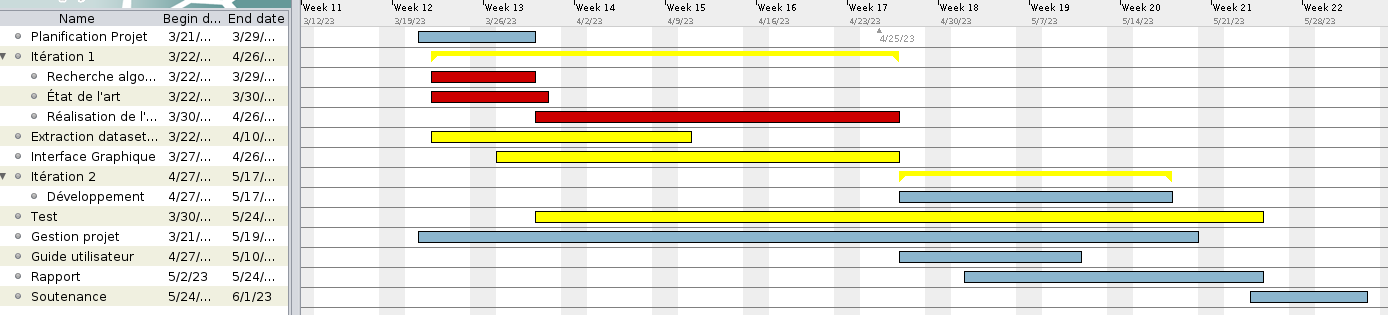
\includegraphics[scale=0.5, angle=90]{gantt.png}


\end{document}
